%
% This is a borrowed LaTeX template file for lecture notes for CS267,
% Applications of Parallel Computing, UCBerkeley EECS Department.
% Now being used for CMU's 10725 Fall 2012 Optimization course
% taught by Geoff Gordon and Ryan Tibshirani.  When preparing
% LaTeX notes for this class, please use this template.
%
% To familiarize yourself with this template, the body contains
% some examples of its use.  Look them over.  Then you can
% run LaTeX on this file.  After you have LaTeXed this file then
% you can look over the result either by printing it out with
% dvips or using xdvi. "pdflatex template.tex" should also work.
%

\documentclass[UTF8,oneside]{article}

% \usepackage[UTF8,scheme=plain]{ctex}
\usepackage[AutoFakeBold,AutoFakeSlant,CJKecglue]{xeCJK}  % 载入 xeCJK以支持中文,支持伪粗体,伪斜体 , 去掉CJK 文字与西文字体间的空格
\usepackage[margin=1in]{geometry}
\usepackage{amsmath,amsthm,amssymb}
\usepackage{graphicx}
\usepackage{autobreak}
\usepackage{tikz}
\usetikzlibrary{positioning} %为了实现相对位置的设定
\usepackage{xcolor} %为了实现不同的颜色
\setCJKmainfont{宋体}                                         % 设置中文中文字体
\setCJKmonofont{宋体}                                        % 设置中文等宽字体
% \setCJKsansfont{宋体}
% \setCJKmainfont{SimSun}[BoldFont=SimHei, ItalicFont=KaiTi]
\setlength{\oddsidemargin}{0.25 in}
\setlength{\evensidemargin}{-0.25 in}
\setlength{\topmargin}{-0.6 in}
\setlength{\textwidth}{6.5 in}
\setlength{\textheight}{8.5 in}
\setlength{\headsep}{0.75 in}
\setlength{\parindent}{0 in}
\setlength{\parskip}{0.1 in}

%
% ADD PACKAGES here:
%

\usepackage{amsmath,amsfonts,graphicx}

%
% The following commands set up the lecnum (lecture number)
% counter and make various numbering schemes work relative
% to the lecture number.
%
\newcounter{lecnum}
\renewcommand{\thepage}{\thelecnum-\arabic{page}}
\renewcommand{\thesection}{\thelecnum.\arabic{section}}
\renewcommand{\theequation}{\thelecnum.\arabic{equation}}
\renewcommand{\thefigure}{\thelecnum.\arabic{figure}}
\renewcommand{\thetable}{\thelecnum.\arabic{table}}

%
% The following macro is used to generate the header.
%
\newcommand{\lecture}[4]{
   \pagestyle{myheadings}
   \thispagestyle{plain}
   \newpage
   \setcounter{lecnum}{#1}
   \setcounter{page}{1}
   \noindent
   \begin{center}
   \framebox{
      \vbox{\vspace{2mm}
    \hbox to 6.28in { {\bf Fundamentals Of Information Science
	\hfill 2022 Spring} }
       \vspace{4mm}
       \hbox to 6.28in { {\Large \hfill   #2  \hfill} }
       \vspace{2mm}
       \hbox to 6.28in { {\it 学生: #3 \hfill 时间: #4} }
      \vspace{2mm}}
   }
   \end{center}
   \markboth{Lecture #1: #2}{Lecture #1: #2}

}
%
% Convention for citations is authors' initials followed by the year.
% For example, to cite a paper by Leighton and Maggs you would type
% \cite{LM89}, and to cite a paper by Strassen you would type \cite{S69}.
% (To avoid bibliography problems, for now we redefine the \cite command.)
% Also commands that create a suitable format for the reference list.
\renewcommand{\cite}[1]{[#1]}
\def\beginrefs{\begin{list}%
        {[\arabic{equation}]}{\usecounter{equation}
         \setlength{\leftmargin}{2.0truecm}\setlength{\labelsep}{0.4truecm}%
         \setlength{\labelwidth}{1.6truecm}}}
\def\endrefs{\end{list}}
\def\bibentry#1{\item[\hbox{[#1]}]}

%Use this command for a figure; it puts a figure in wherever you want it.
%usage: \fig{NUMBER}{SPACE-IN-INCHES}{CAPTION}
\newcommand{\fig}[3]{
			\vspace{#2}
			\begin{center}
			Figure \thelecnum.#1:~#3
			\end{center}
	}
% Use these for theorems, lemmas, proofs, etc.
\usepackage{amsthm}
\newtheorem*{Solution}{Solution}
\newtheorem{theorem}{Theorem}[lecnum]
\newtheorem{lemma}[theorem]{Lemma}

\newtheorem{proposition}[theorem]{Proposition}
\newtheorem{claim}[theorem]{Claim}
\newtheorem{corollary}[theorem]{Corollary}
\newtheorem{definition}[theorem]{Definition}
% \newenvironment{proof}{{\bf Proof:}}{\hfill\rule{2mm}{2mm}}

% **** IF YOU WANT TO DEFINE ADDITIONAL MACROS FOR YOURSELF, PUT THEM HERE:

\newcommand\E{\mathbb{E}}

\begin{document}
%FILL IN THE RIGHT INFO.
%\lecture{**LECTURE-NUMBER**}{**DATE**}{**LECTURER**}{**SCRIBE**}
\lecture{1}{Homework2}{华园(202000120027))}{2022.3.3}
%\footnotetext{These notes are partially based on those of Nigel Mansell.}

% **** YOUR NOTES GO HERE:

% Some general latex examples and examples making use of the
% macros follow.
%**** IN GENERAL, BE BRIEF. LONG SCRIBE NOTES, NO MATTER HOW WELL WRITTEN,
%**** ARE NEVER READ BY ANYBODY.

\section*{Problem 1.} % Don't be this informal in your notes!
(a)Construct a circuit with 3 relays that implements the functions
\begin{align*}

f_1&=x·y		\\
f_2&=\overline{x}·y
\end{align*}

\begin{Solution}
\end{Solution}
\begin{center}
  \begin{tikzpicture}
\draw  [black,->](0,0)--node[below=-5pt,fill=white]{$y$}(-3,0);
\draw  [black](0,0)--node[below=-5pt,fill=white]{$x$}(2,2);
\draw  [black](0,0)--node[below=-5pt,fill=white]{$\overline{x}$}(2,-2);
\filldraw [red] (2,2) circle (2pt)--node[right=4pt,fill=white]{$f_1$}(2,2);
\filldraw [blue] (2,-2) circle (2pt)--node[right=4pt,fill=white]{$f_2$}(2,-2);
\filldraw [black] (-3,0) circle (2pt);

  \end{tikzpicture}
\end{center}
(b)Construct a circuit with 4 relays that implements the functions
\begin{align*}

f_1&=x·y+\overline{x}·\overline{y}	\\
f_2&=\overline{x}·y+x·\overline{y}
\end{align*}
\begin{Solution}
\end{Solution}
\begin{center}
  \begin{tikzpicture}
\draw  [black](0,-3)--node[below=-5pt,fill=white]{$\overline{y}$}(-3,0);
\draw  [black](-3,0)--node[below=-5pt,fill=white]{$x$}(0,3);
\draw  [black](0,3)--node[below=-5pt,fill=white]{$y$}(3,0);
\draw  [black](3,0)--node[below=-5pt,fill=white]{$\overline{x}$}(0,-3);
\filldraw [red] (-3,0) circle (2pt)--node[left=4pt,fill=white]{$f_1$}(-3,0);
\filldraw [red] (3,0) circle (2pt)--node[right=4pt,fill=white]{$f_1$}(3,0);
\filldraw [blue] (0,-3) circle (2pt)--node[right=5pt,fill=white]{$f_2$}(0,-3);
\filldraw [blue] (0,3) circle (2pt)--node[right=5pt,fill=white]{$f_2$}(0,3);

  \end{tikzpicture}
\end{center}

(c)Construct a circuit with 6 relays that implements the functions
\begin{align*}

f_1&=x·(y+z)\\
f_2&=y·(x+z)\\
f_3&=z·(x+y)\\
f_4&=x+y·z\\
f_5&=y+x·z\\
f_6&=z+x·y\\
\end{align*}
\begin{Solution}
\end{Solution}
\begin{center}
  \begin{tikzpicture}
\draw  [black](0,1.3)--node[below=-5pt,fill=white]{$y$}(1.5,-1.3);
\draw  [black](1.5,-1.3)--node[below=-5pt,fill=white]{$x$}(-1.5,-1.3);
\draw  [black](-1.5,-1.3)--node[below=-5pt,fill=white]{$z$}(0,1.3);
\draw  [black](0,1.3)--node[below=-5pt,fill=white]{$x$}(0,2.5);
\draw  [black](1.5,-1.3)--node[below=-5pt,fill=white]{$z$}(2.5,-2.16);
\draw  [black](-1.5,-1.3)--node[below=-5pt,fill=white]{$y$}(-2.5,-2.16);
\filldraw [red] (0,2.5) circle (2pt)--node[right=4pt,fill=white]{$f_1$}(0,2.5);
\filldraw [blue] (-2.5,-2.16) circle (2pt)--node[left=4pt,fill=white]{$f_2$}(-2.5,-2.16);
\filldraw [orange] (2.5,-2.16) circle (2pt)--node[right=4pt,fill=white]{$f_3$}(2.5,-2.16);
\draw  [blue, very thick](0,1.3)--(3,1.3);
\draw  [orange,very thick](0,1.3)--(-3,1.3);
\draw  [orange,very thick](-1.5,-1.3)--(-3,1.3);
\draw  [blue,very thick](1.5,-1.3)--(3,1.3);
\draw  [red,very thick](1.5,-1.3)--(0,-3.9);
\draw  [red,very thick](-1.5,-1.3)--(0,-3.9);
\filldraw [red] (0,-3.9) circle (2pt)--node[right=4pt,fill=white]{$f_1$}(0,-3.9);
\filldraw [blue] (3,1.3) circle (2pt)--node[right=4pt,fill=white]{$f_2$}(3,1.3);
\filldraw [orange] (-3,1.3) circle (2pt)--node[left=4pt,fill=white]{$f_3$}(-3,1.3);
\draw  [yellow,,very thick](1.5,-2)--(1.5,-1.3);
\draw  [yellow,,very thick](-1.5,-2)--(-1.5,-1.3);
\filldraw [yellow] (-1.5,-2.) circle (2pt)--node[below=4pt,fill=white]{$f_4$}(-1.5,-2);
\filldraw [yellow] (1.5,-2) circle (2pt)--node[below=4pt,fill=white]{$f_4$}(1.5,-2);
\draw  [green,,very thick](1.5,-1.3)--(2.3,-1.3);
\draw  [green,,very thick](0,1.3)--(0.5,2);
\filldraw [green] (2.3,-1.3) circle (2pt)--node[right=4pt,fill=white]{$f_5$}(2.3,-1.3);
\filldraw [green] (0.5,2) circle (2pt)--node[right=4pt,fill=white]{$f_5$}(0.5,2);
\draw  [black,,very thick](-1.5,-1.3)--(-2.3,-1.3);
\draw  [black,,very thick](0,1.3)--(-0.5,2);
\filldraw [black] (-2.3,-1.3) circle (2pt)--node[left=4pt,fill=white]{$f_6$}(-2.3,-1.3);
\filldraw [black] (-0.5,2) circle (2pt)--node[left=4pt,fill=white]{$f_6$}(-0.5,2);
  \end{tikzpicture}
\end{center}




\section*{Problem 2.}
You are asked to design a Turing machine that accepts the following languages:some number of 1's followed by the same number of 0’s.\\
\begin{center}
 [\#10\#,\#1100\#,\#111000\#,\#11110000\#,...]
\end{center}
Explain your design.
\begin{Solution}
\end{Solution}
\begin{center}
  \begin{tikzpicture}

\filldraw[color=black, fill=white, very thick] (0,0) circle (1)--node[below=-7pt,fill=white,thick]{$Check\,1$}(0,0);
\filldraw[color=black, fill=white, very thick] (5,0) circle (1)--node[below=-7pt,fill=white]{$GO\, to\,end$}(5,0);
\filldraw[color=black, fill=white, very thick] (5,4) circle (1)--node[below=-7pt,fill=white]{$clear\,a\,0$}(5,4);
\filldraw[color=black, fill=white, very thick] (0,4) circle (1)--node[below=-7pt,fill=white]{$GO\, start$}(0,4);
\filldraw[color=red, fill=white, very thick] (-5,0) circle (1)--node[below=-7pt,fill=white]{$Reject$}(-5,0);
\draw  [black,very thick,->](1,0)--node[below=09pt,fill=white]{$(1\rightarrow\#)/R$}(4,0);
\draw  [black,very thick,->](0,3)--node[right=10pt,fill=white]{$(\#\rightarrow\#)/R$}(0,1);
\draw  [black,very thick,->](5,1)--node[right=7pt,fill=white]{$(\#\rightarrow\#)/L$}(5,3);
\draw  [black,very thick,->](4,4)--node[below=5pt,fill=white]{$(0\rightarrow\#)/L$}(1,4);
\draw  [black,very thick,->](-1,0)--node[below=5pt,fill=white]{$(0\rightarrow\#)/R$}(-4,0);
\draw  [black,very thick,](5,5)--(5,6.2);
\draw  [black,very thick,->](0,-1)--node[left=10pt,fill=white]{$(\#\rightarrow\#)/R$}(0,-2);
\draw  [black,very thick,->](-5,6.2)--(-5,1);
\draw  [black,very thick,](5,6.2)--node[below=-15pt,fill=white]{$(1\rightarrow1)/R$}(-5,6.2);
\draw  [black,very thick,](5,6.2)--node[below=-30pt,fill=white]{$(\#\rightarrow\#)/R$}(-5,6.2);
\draw[very thick , ->](5, -1) arc (-180:90:1);
\draw  [black,->](7,-1)--node[below=0pt,fill=white]{$1\rightarrow 1)/R$}(7,-1);
\draw  [black,->](7,-1)--node[below=-15pt,fill=white]{$0\rightarrow 0)/R$}(7,-1);
\draw  [black,->](-2,5)--node[below=0pt,fill=white]{$(1\rightarrow 1)/L$}(-2,5);
\draw  [black,->](-2,5)--node[below=-15pt,fill=white]{$(0\rightarrow 0)/L$}(-2,5);
\draw[very thick , ->](0, 5) arc (0:270:1);
	\filldraw[color=green, fill=white, very thick] (0,-3) circle (1)--node[below=-7pt,fill=white]{$Accept$}(0,-3);
  \end{tikzpicture}
\end{center}

\section*{Problem 3.}
(1)write CQ(X) with 6 inputs function|	X|. Note that there 7 entries in the table.\\
\begin{Solution}

\end{Solution}
	\begin{table}[h]
\centering
\begin{tabular}{|c|c|}
\hline
|X| & CQ(X)\\
\hline
0 & 0 \\
\hline
1 & 0	\\
\hline
2 & 1	\\
\hline
3 & 1 \\
\hline
4 & 0\\
\hline
5 & 0\\
\hline
6 & 1\\
\hline
\end{tabular}
\label{TAB1}
\end{table}
(2)For an arbitrary n,express CQ(X) as a function of |X|. Namely,you need to specify,as a mathematical expression,the value of |X| for whick CQ(X)=1,Jusify your solution. 
\begin{Solution}
\end{Solution}
XOR is a symmetric function,when the number of 1 in the input is odd, the output is 1.thus:
\begin{center}
\begin{align*}
when:\qquad C_{|x|}^{2}=\frac{|x|·(|x|-1)}{2}&=2k+1\qquad(|x|\geq2,k \in N)\\
CQ(X)&=1
\end{align*}
\end{center}


% **** THIS ENDS THE EXAMPLES. DON'T DELETE THE FOLLOWING LINE:

\end{document}





